\section{Experiments}\label{sec:exp}
All numbers below are produced by the scripts listed in the reproduction notes (Appendix~\ref{app:repro}) from the committed result files; $\alpha=0.1$ is the primary level. A \emph{replicate} is an independent draw of data, predictor fit, calibration split and test set; intervals are $95\%$ $t$-intervals of the mean over replicates unless stated.

\subsection{Setup}
\paragraph{Synthetic worlds (E1).} $x\sim\mathcal N(0,I_4)$, mean $\mu(x)=\mathrm{softmax}(Bx+b)$ with a fixed random $(B,b)$ per configuration, $K\in\{3,5,10\}$. The conditional law is Dirichlet ($y\sim\mathrm{Dir}(\phi\mu)$, $\phi=20/h(x)$), logistic-normal ($y=\mathrm{softmax}(\log\mu+0.5\,h(x)\varepsilon)$), multinomial proportions ($30/h(x)$ counts, hence exact zeros) or a rounded logistic-normal with parts below $0.01$ set to zero. The noise factor is $h\equiv1$ (homoscedastic) or $h(x)=\exp(0.8\,w^\top x)$ (heteroscedastic). Predictors are a multinomial-logit regression on soft labels (the correct mean model for Dirichlet and multinomial noise, misspecified for the logistic-normal) and a random forest. Each replicate uses $1000$ points to fit, $500$ to fit $\hat\sigma$ and $\hat\phi$, $n$ calibration points (default $500$) and $2000$ test points.
\paragraph{Real data.} E2: a small CNN trained on CIFAR-10, with the test set split at random into calibration ($n=1000$) and test points, $200$ splits; label sets from the scores evaluated at the vertices. Two checkpoints (2 and 12 epochs; accuracy $0.740$ and $0.881$) vary the predictor's quality.

\subsection{Validity is score-free: the Beta law (C1)}
For each of three scores and two noise laws ($K=5$, linear predictor) we draw $3000$ calibration sets of size $n\in\{19,50,100,500\}$ and evaluate the calibration-conditional coverage on a test pool of $2\cdot10^6$ points. Fig.~\ref{fig:beta} shows the empirical mean and $5/95\%$ quantiles against the Beta band of Proposition~\ref{prop:beta}. The largest deviation of an empirical mean from the Beta mean over the $24$ cells is $0.002$; Kolmogorov--Smirnov $p$-values are $0.03$--$0.98$ (Dirichlet) and $0.02$--$0.86$ (multinomial), with $3$ of $24$ below $0.05$, consistent with chance given $24$ tests of which none is corrected. Note that this check uses the continuous noise laws; with exact zeros (E3, rounded worlds) ties only give the lower bound.
\begin{figure}[tbp]
\centering
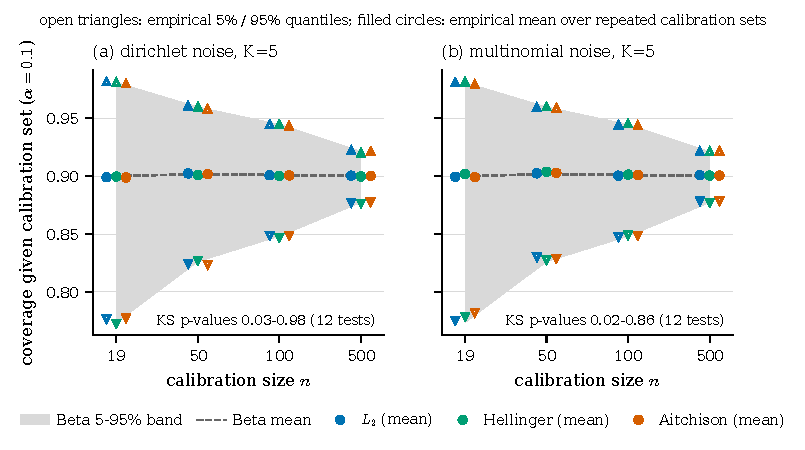
\includegraphics[width=0.85\linewidth]{fig1_beta_law.pdf}
\caption{Calibration-conditional coverage of split conformal prediction ($\alpha=0.1$, $K=5$, linear predictor) over $3000$ calibration sets per cell, for $L_2$, Hellinger and Aitchison scores. Shaded: exact $5$--$95\%$ band of $\mathrm{Beta}(k,n+1-k)$; markers: empirical mean and $5/95\%$ quantiles. KS $p$-values over the $12$ cells of each panel are annotated.}\label{fig:beta}
\end{figure}

\subsection{Efficiency of the regions depends on the score and on the noise law (C2)}
All $15$ main variants and CV+ are marginally valid in all $48$ configurations (mean coverage $0.896$--$0.909$), so differences in size compare equally valid regions. As efficiency measure we use the region \emph{mass} $\texttt{pool\_frac}$: the share of the marginal law of $y$ inside the region, estimated on the test pool. It is defined for every $K$, unlike the Lebesgue volume, which we compute only for $K\le5$ (Appendix, Fig.~\ref{fig:sizevol}; the Spearman correlation between mass and volume is $0.89$ at $K=3$ and $0.96$ at $K=5$). Fig.~\ref{fig:size} gives the mass relative to the plain $L_2$ region of the same replicate, for heteroscedastic worlds with a linear predictor.
\begin{figure}[tbp]
\centering
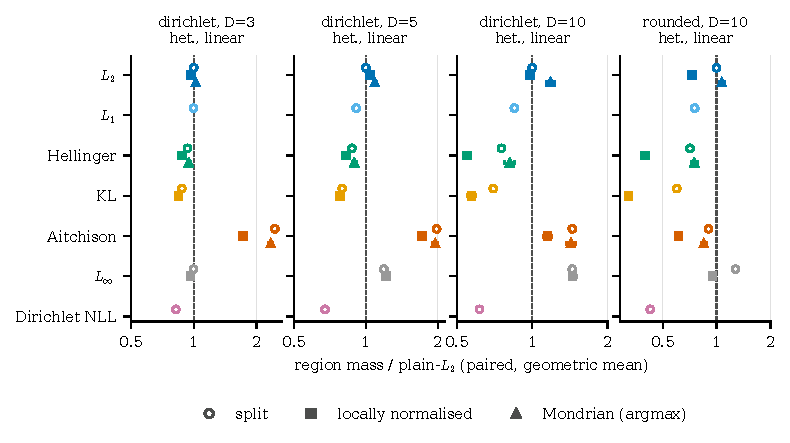
\includegraphics[width=0.85\linewidth]{fig2_size.pdf}
\caption{Region mass relative to the plain $L_2$ region of the same replicate (geometric mean over $100$ replicates; $95\%$ $t$-interval of the log ratio, mostly smaller than the markers), $\alpha=0.1$, $n_{\mathrm{cal}}=500$, heteroscedastic, linear predictor. Below $1$: more informative at equal coverage. Open: plain split; squares: locally normalised; triangles: Mondrian (argmax).}\label{fig:size}
\end{figure}
Three patterns stand out. (i) The ranking of scores is not stable across noise laws. The plain Aitchison region is $2.45$, $1.98$ and $1.45$ times the plain $L_2$ region for Dirichlet noise at $K=3,5,10$, but $0.90$ times for the rounded logistic-normal at $K=10$. (ii) The Dirichlet NLL score gives the smallest region in every Dirichlet panel ($0.82$, $0.67$, $0.62$ of $L_2$); the information-based scores follow (KL $0.88$, $0.80$, $0.70$; Hellinger $0.93$, $0.87$, $0.75$), whereas $L_\infty$ is no better than $L_2$ and worse for larger $K$ ($1.19$, $1.44$ at $K=5,10$). (iii) Local normalisation can shrink regions strongly at $K=10$ (normalised KL: $0.57$ of plain $L_2$ for Dirichlet noise and $0.32$ for the rounded world). Table~\ref{tab:e1} (Appendix~\ref{app:more}) gives all variants for $K=5$.

\subsection{Conditional coverage: normalisation helps under heteroscedasticity only (C3)}
Fig.~\ref{fig:cond} shows four conditional-coverage metrics at $K=5$, $n_{\mathrm{cal}}=500$, with the null band of Fig.~\ref{fig:null} in grey: the oracle gap $\overline{|c(x)-0.9|}$ from the known generator, the gap between the best and worst of five bins of the predicted top probability, worst-slab coverage, and coverage given $y$ near the boundary of the simplex (outcome-conditional and descriptive only).
\begin{figure}[tbp]
\centering
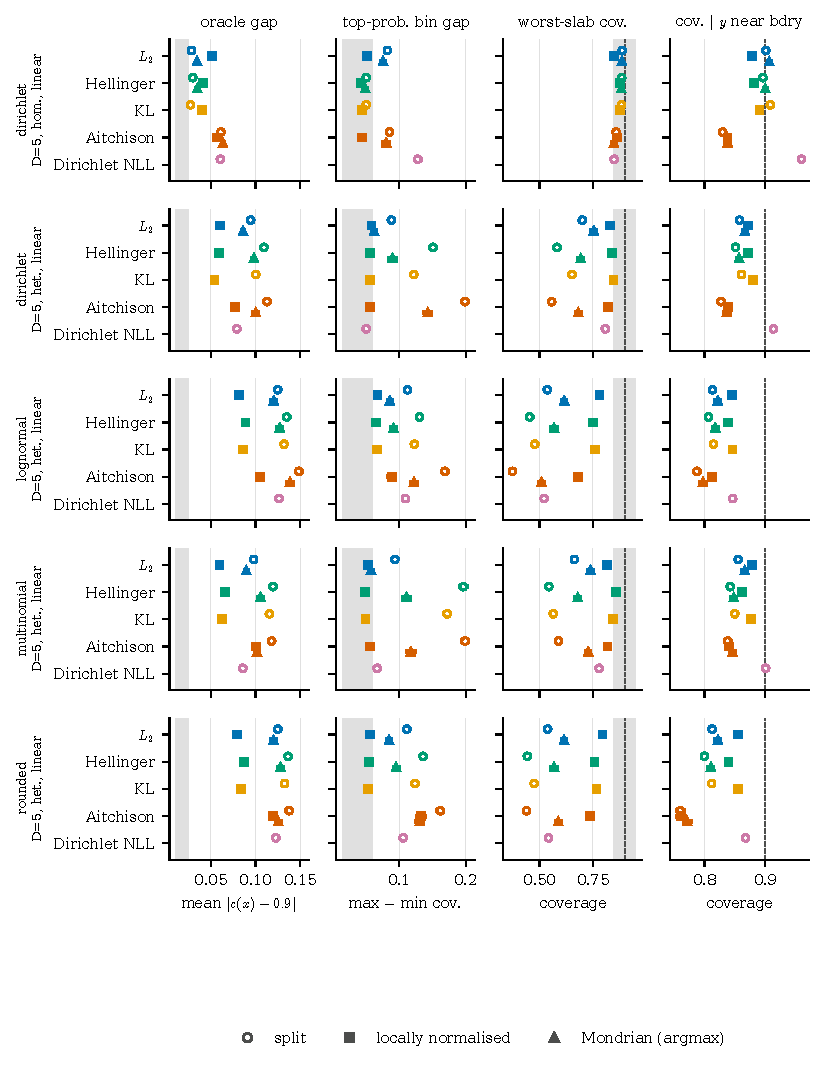
\includegraphics[width=\linewidth,height=0.42\textheight,keepaspectratio]{fig3_conditional.pdf}
\caption{Conditional-coverage metrics in five $K=5$ worlds ($n_{\mathrm{cal}}=500$, linear predictor, $100$ replicates; the $95\%$ intervals are smaller than the markers). Grey: $5$--$95\%$ band of the metric when conditional coverage is exact (Fig.~\ref{fig:null}); dashed: nominal $0.9$. Markers as in Fig.~\ref{fig:size}.}\label{fig:cond}
\end{figure}
Under homoscedastic Dirichlet noise the oracle gap of the $L_2$, $L_1$, $L_\infty$, Hellinger and KL scores is $0.026$--$0.030$, just above the null band ($0.011$--$0.025$), and local normalisation does not help (over the $24$ homoscedastic configurations the normalised score has the smaller gap in only $8$, with means $0.070$ against $0.062$). Under heteroscedastic noise every plain score is far from the null: the oracle gap is $0.079$--$0.148$ and worst-slab coverage as low as $0.37$--$0.60$, e.g. plain $L_2$ $0.118$ and $0.60$ against $0.083$ and $0.82$ for its normalised variant, which is better in all $24$ heteroscedastic configurations. Even the best variant (Dirichlet: normalised KL, gap $0.054$, wsc $0.85$; logistic-normal: normalised $L_\infty$, $0.077$, $0.81$) stays far above the floor, so normalisation by an estimated scale reduces but does not remove conditional miscoverage. The plain Aitchison score has the lowest worst-slab coverage in three of the four heteroscedastic rows ($0.56$ Dirichlet, $0.37$ logistic-normal, $0.44$ rounded; in the multinomial row Hellinger $0.54$ and Aitchison $0.59$ are lowest), and the plain Dirichlet NLL score is the best plain score only in its own world ($0.079$, wsc $0.81$; in the logistic-normal world its gap equals that of $L_2$, $0.126$ against $0.125$). Mondrian regions by argmax of the prediction improve plain scores less than scale normalisation (Table~\ref{tab:e1}). So no score is uniformly the best on both size and conditional coverage: the smallest mass is achieved by the Dirichlet NLL in its own world ($0.11$) but by normalised Aitchison ($0.21$, with a gap $0.105$) in the logistic-normal world.

\subsection{Calibration size and calibration scheme (C4)}
Fig.~\ref{fig:ncal} (Appendix~\ref{app:more}) varies $n_{\mathrm{cal}}\in\{30,100,250,500,2000\}$ ($K=5$, heteroscedastic, linear predictor). The standard deviation of test coverage over replicates follows $\sqrt{\mathrm{Var}\,\mathrm{Beta}(k,n+1-k)+0.09/2000}$, the Beta spread plus test-set noise, for all three scores shown, so the finite-sample coverage fluctuation is score-free also in this setting and shrinks from about $0.05$ to $0.01$. Region size behaves differently by scheme. Mondrian calibration by argmax needs enough points per group: at $n_{\mathrm{cal}}=30$ the threshold is infinite for $47\%$ of test points (the region is the whole simplex), coverage is $0.96$--$0.95$, and the median region volume is $0.73$ (Dirichlet) and $0.90$ (logistic-normal) against $0.13$ and $0.53$ for plain split; the difference is gone at $n_{\mathrm{cal}}=250$ in the Dirichlet world, and at $n_{\mathrm{cal}}=2000$ Mondrian is slightly smaller than plain split ($0.09$ against $0.11$; $0.38$ against $0.42$) but, for logistic-normal noise, not than the normalised variant. The locally normalised variant is stable in $n_{\mathrm{cal}}$ in these worlds; in the logistic-normal world it halves the region ($0.21$ against $0.53$ at $n_{\mathrm{cal}}=30$, $0.18$ against $0.42$ at $2000$). CV+ ($L_2$) has near-constant volume ($0.10$ and $0.42$) with coverage $0.90$ at every $n_{\mathrm{cal}}$; because it pools fitting and calibration data, its $n_{\mathrm{cal}}$ is not on the same footing as split conformal prediction, and CV+ was run for the linear predictor only.

\subsection{Zero replacement for the Aitchison score}
The Aitchison score needs parts replaced by $\varepsilon>0$. Marginal coverage is unaffected ($0.896$--$0.909$ for all plotted variants) but the region mass of the plain score falls from $0.52$--$0.63$ at $\varepsilon=10^{-4}$ to $0.13$--$0.31$ at $\varepsilon=0.1$ (Dirichlet $0.52\to0.14$, multinomial $0.57\to0.13$, rounded $0.63\to0.31$), while worst-slab coverage moves little and non-monotonically and stays below that of normalised $L_2$ (Fig.~\ref{fig:eps}, Appendix). The zero-replacement constant is therefore a tuning parameter of efficiency that must be reported; here the main grid used $\varepsilon=10^{-3}$.

\subsection{Label-set bridge on CIFAR-10 (C7)}
Table~\ref{tab:e2} gives results at $T=1$. All methods reach $0.900$ marginal coverage, as Proposition~\ref{prop:beta} implies. As Proposition~\ref{prop:vertex} states, $L_1$, Hellinger and KL sets are identical to LAC sets in $100\%$ of test points (column ``$=$LAC''), so these three are not different methods on classifier outputs; the Brier ($L_2$) and Aitchison sets differ from LAC in $2.8\%$ and $2$--$9\%$ of points at $12$ epochs. LAC has the smallest sets ($1.055$) but the largest class-conditional undercoverage (minimum per-class coverage $0.800$ against $0.872$ for APS at size $1.303$), which is the usual efficiency--adaptivity trade-off \citep{angelopoulos2021raps}. Which score is better on SSCV depends on the checkpoint and zero replacement: with $\varepsilon=10^{-3}$ the Aitchison score reaches SSCV$^\dagger$ $0.911$ at $12$ epochs but produces $2.6\%$ empty sets and a lower minimum class coverage ($0.794$), whereas $\varepsilon=0.1$ gives $0.814$; the Aitchison score on a softmax is thus sensitive to the zero-replacement constant.
\begin{table}[tbp]
\centering\small
\caption{CIFAR-10 label sets, $T=1$, $n_{\mathrm{cal}}=1000$, $200$ random calibration/test splits of the $10{,}000$ test images; mean $\pm$ half-width of the $95\%$ $t$-interval over splits. SSCV$^\dagger$: minimum coverage over size strata $\{1\},\{2\text{--}3\},\{4{+}\}$ (strata with fewer than $30$ points dropped). ``$=$LAC'': share of test points whose set equals the LAC set.}\label{tab:e2}
\resizebox{\linewidth}{!}{\input{../tables/tab3_e2_labelsets}}
\end{table}

\subsection{Conditional coverage under Dirichlet noise: where the first-order theory holds (C6)}
Fig.~\ref{fig:delta} (Appendix~\ref{app:more}) compares the delta-method prediction of Section~\ref{sec:theory} with simulated pointwise coverage (oracle mean predictor, $300$ values of $x$ per panel, precision $\phi\in\{200,50,20,8\}$). For the Euclidean score the prediction is accurate (RMSE $0.008$--$0.010$ across all four precisions; correlation $\ge0.94$). For the Hellinger score the first-order prediction is exactly flat at $0.9$ (the Gaussian approximation is variance-stabilised, which is why no correlation is defined), while the simulated coverage varies in $[0.81,0.99]$ with RMSE $0.014$--$0.038$ growing as $\phi$ falls; we only learn that Hellinger conditional coverage is much closer to homogeneous than Euclidean, not by how much. For the Aitchison score the approximation fails (RMSE $0.16$--$0.27$; correlation $0.58$ at $\phi=200$ falling to $-0.44$ at $\phi=8$, also for a second-order moment variant): we conjecture that the log-ratio score is dominated by the smallest parts, where the Gaussian approximation of a Dirichlet is poor, but we did not test this. We therefore claim the first-order prediction only for the Euclidean score in the tested range $\phi\ge8$, $K=5$.

\subsection{How large must a difference in conditional-coverage metrics be? (C5)}
Binned and worst-slab metrics are noisy and, being extrema over bins or slabs, biased even for a method with exact conditional coverage. We quantify this by a null simulation: for each $n_{\mathrm{cal}}$ we draw $500$ replicates in which the coverage level is $p\sim\mathrm{Beta}(k,n+1-k)$ (the exact split-conformal law) and coverage indicators on $2000$ test points are Bernoulli$(p)$ independent of the features, then apply the same binning and slab code as in E1 (Fig.~\ref{fig:null}). At $n_{\mathrm{cal}}=500$ the null gap between the highest and lowest of $5$ equal-mass bins of the predicted maximal part is $0.034$ (sd $0.013$), the null worst-slab coverage is $0.90$ (sd $0.03$), and the oracle pointwise gap (60 points, $400$ draws each) has a floor of $0.016$ (sd $0.005$) from Monte-Carlo noise and the calibration-induced deviation of $p$ from $0.9$. A difference between methods below these spreads is not interpretable, and we report conditional-coverage gaps in the following section only relative to this null band.
\begin{figure}[tbp]
\centering
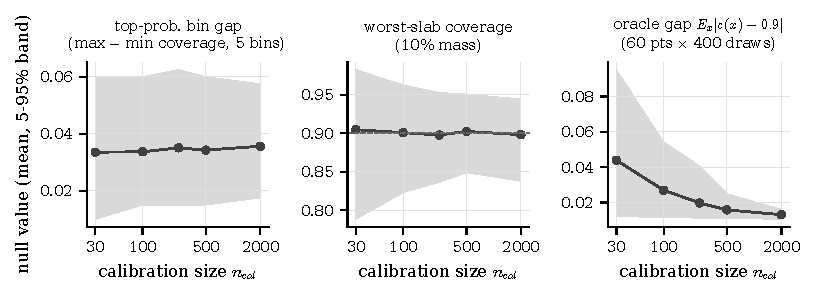
\includegraphics[width=0.85\linewidth]{fig5_null_spread.pdf}
\caption{Null distribution of three conditional-coverage metrics when conditional coverage is exact by construction ($n_{\mathrm{test}}=2000$, $500$ replicates per $n_{\mathrm{cal}}$). Line: mean; band: $5$--$95\%$.}\label{fig:null}
\end{figure}

\subsection{A real composition-valued response: CIFAR-10H (C8)}
CIFAR-10H gives, for each CIFAR-10 test image, the distribution of human labels, a composition with $80.6\%$ exact zeros; the predictor is the $12$-epoch CNN softmax ($T=1$). Because of the zeros and discrete vote proportions, scores tie and Proposition~\ref{prop:beta} guarantees only $\ge1-\alpha$; coverage refers to the noisy vote proportions, not to a latent label law. Dimension is $K=10$, so the Lebesgue volume is useless; as efficiency we use ``mass'', the share of the other images' human distributions that fall inside the region (lower is more informative at equal coverage). Table~\ref{tab:e3} (Appendix~\ref{app:more}; 100 random splits into $2000$/$1000$/rest for $\hat\sigma$, calibration and test) shows: (i) all $18$ variants reach marginal coverage $0.900$--$0.906$, slightly above $0.9$ for Mondrian ($0.905$--$0.906$), consistent with ties and small groups; (ii) plain and Mondrian regions have similar mass ($0.103$--$0.118$) for all scores, whereas locally normalised regions are $3$--$5$ times less informative ($0.32$--$0.56$) and do not repair conditional coverage; (iii) coverage in the worst of five confidence bins of the CNN stays at $0.63$--$0.75$ for every variant, far below $0.9$ and far outside the null band of Fig.~\ref{fig:null} (gap $0.034$); the entropy of the human distribution is an outcome-conditional diagnostic, not a conditioning variable of the guarantee, so its bin gaps need not vanish. We cannot rank scores on this dataset beyond this: the intervals of several rows overlap, and the single predictor, single dataset and tie structure limit what transfers.

\subsection{Covariate shift: a bounded check (C10)}
Section~\ref{sec:disc} excludes shift from the guarantees, but we check one family: $K=5$, heteroscedastic, linear predictor, calibration $x\sim\mathcal N(0,I)$ and test $x\sim\mathcal N(\delta w,I)$ with $w$ the direction of increasing noise, $n_{\mathrm{cal}}=500$, $100$ replicates. Fig.~\ref{fig:shift} (Appendix~\ref{app:more}) shows that ordinary split conformal prediction loses coverage as $\delta$ grows: at $\delta=1.5$ the plain scores fall to $0.49$--$0.73$ (logistic-normal $0.49$--$0.59$) and the locally normalised ones to $0.70$--$0.92$, so normalisation mitigates but does not remove the loss. Weighted split conformal prediction with the exact likelihood ratio \citep{tibshirani2019covariate} restores coverage to $0.895$--$0.920$ in all families and shifts, at the price of a smaller effective calibration size (down to $73$ at $\delta=1.5$). The exact likelihood ratio is known here; with estimated weights this is not guaranteed. This is one shift family on one predictor and supports no general statement about shift.
